\documentclass[conference]{IEEEtran}
\IEEEoverridecommandlockouts

% ---------------------------------------------------------------
% Pacotes
% ---------------------------------------------------------------
\usepackage[utf8]{inputenc}
\usepackage[T1]{fontenc}
\usepackage[brazil]{babel}
\usepackage{cite}
\usepackage{amsmath,amssymb,amsfonts}
\usepackage{graphicx}
\usepackage{textcomp}
\usepackage{xcolor}
\usepackage{booktabs}
\usepackage{array}
\usepackage{url}
\usepackage{tikz}
\usetikzlibrary{arrows.meta,positioning}

\graphicspath{{figuras/}}
\renewcommand{\IEEEkeywordsname}{Palavras-chave}

\begin{document}

% ---------------------------------------------------------------
% Título
% ---------------------------------------------------------------
\title{Identificação de Espécies de Aves pelo Canto com Aprendizagem Profunda: CNNs, Redes Recorrentes e Modelos de Áudio Pré-Treinados\\[4pt]
\large Relatório Final --- CIN0040 Introdução à Aprendizagem Profunda}

\author{
\IEEEauthorblockN{Giovanny Lira de Araujo Cunha}
\IEEEauthorblockA{\textit{Centro de Informática (CIn)} \\
\textit{Universidade Federal de Pernambuco}\\
Recife, Brasil \\
glac2@cin.ufpe.br}
\and
\IEEEauthorblockN{Caio Henrique Araujo Braga}
\IEEEauthorblockA{\textit{Centro de Informática (CIn)} \\
\textit{Universidade Federal de Pernambuco}\\
Recife, Brasil \\
chab@cin.ufpe.br}
}

\maketitle

% ---------------------------------------------------------------
\begin{abstract}
Este trabalho compara famílias de redes profundas na classificação de 20 espécies de aves a partir de trechos de 5~s de áudio, usando um subconjunto equilibrado do BirdCLEF 2025 (3000 gravações do xeno-canto). Sob um protocolo único, com divisão agrupada por gravação, validação cruzada de 5 \textit{folds} e um teste fixo de 600 gravações, avaliamos uma CNN e uma CRNN treinadas do zero, o PANNs CNN14 com ajuste fino e o Audio Spectrogram Transformer congelado. O CNN14 obteve F1-macro de $0{,}938 \pm 0{,}008$, superando a CNN do zero ($0{,}880 \pm 0{,}008$) em todos os \textit{folds}, com vantagem que cresce para 11 pontos quando há só 25\% dos dados; o AST congelado ficou abaixo da CNN ($0{,}824$), e a CRNN não superou a CNN. O aumento de dados (SpecAugment, \textit{mixup} e ruído ambiental) reduziu à metade a queda de desempenho sob ruído a 0~dB. Numa etapa de melhorias, a PCEN como entrada foi a técnica mais eficaz, e uma CNN própria (M6), montada a partir desses resultados, chegou a $0{,}924$ com 0{,}32 milhão de parâmetros, empatando com uma EfficientNet pré-treinada 12 vezes maior. O melhor sistema, um \textit{ensemble} calibrado, atinge F1-macro de $0{,}950$. Discutimos ainda o quanto esses números dependem de dados curados e de gravadores repetidos entre treino e teste.
\end{abstract}

\begin{IEEEkeywords}
bioacústica, classificação de áudio, espectrograma Mel, PCEN, CNN, CRNN, transferência de aprendizado, aumento de dados.
\end{IEEEkeywords}

% ---------------------------------------------------------------
\section{Introdução}

O monitoramento acústico passivo, com gravadores deixados em campo, tornou-se uma ferramenta central para acompanhar a biodiversidade~\cite{stowell2022}. Como esses gravadores produzem milhares de horas de áudio, a identificação manual não escala, e sistemas baseados em redes profundas, como o BirdNET~\cite{kahl2021birdnet}, passaram a automatizar a tarefa. O problema reúne desafios típicos de áudio real: cantos parecidos entre espécies, ruído de fundo e \textbf{rótulos fracos}, já que o rótulo vale para a gravação inteira, mas nem todo trecho contém o canto.

Este trabalho pergunta o que mais contribui para o desempenho nessa tarefa: a arquitetura, o pré-treino em grandes bases de áudio ou o aumento de dados. A proposta definiu três hipóteses:

\begin{itemize}
  \item \textbf{H1:} modelos pré-treinados no AudioSet superam os treinados do zero, sobretudo com poucos dados;
  \item \textbf{H2:} uma CRNN supera uma CNN de mesmo porte;
  \item \textbf{H3:} o aumento de dados reduz a queda de desempenho sob ruído (SNR $\leq 10$~dB).
\end{itemize}

As contribuições são: (i) uma comparação controlada de quatro arquiteturas sob o mesmo \textit{pipeline} e o mesmo protocolo; (ii) experimentos de robustez a ruído e de eficiência de dados; (iii) uma etapa de melhorias com regras explícitas contra o sobreajuste ao conjunto de teste, que registra também as técnicas que falharam; e (iv) uma CNN própria, o M6, cujas peças foram escolhidas a partir desses resultados e avaliadas por ablação. Código, \textit{notebooks}, resultados e pesos estão em \url{https://github.com/Giovanny29/birdclef-dl}.

% ---------------------------------------------------------------
\section{Trabalhos relacionados}

Espectrogramas log-Mel com redes convolucionais são a abordagem padrão em classificação de áudio~\cite{hershey2017}. Redes convolucionais-recorrentes acrescentam uma camada recorrente sobre o eixo do tempo para modelar a sequência de eventos~\cite{choi2017crnn}. O pré-treino em larga escala no AudioSet~\cite{gemmeke2017audioset} produziu modelos como as PANNs~\cite{kong2020panns}, CNNs treinadas em 2 milhões de clipes, e o AST~\cite{gong2021ast}, um \textit{transformer} sobre \textit{patches} do espectrograma. Em bioacústica, o BirdNET~\cite{kahl2021birdnet} e as edições do BirdCLEF~\cite{kahl2021birdclef} consolidaram o uso dessas redes, em geral combinadas com aumento de dados como SpecAugment~\cite{park2019specaugment}, \textit{mixup}~\cite{zhang2018mixup} e mistura de ruído ambiental. A PCEN (\textit{per-channel energy normalization})~\cite{wang2017pcen} é uma alternativa ao logaritmo que normaliza cada banda pela sua energia recente e foi tornada treinável no LEAF~\cite{zeghidour2021leaf}.

% ---------------------------------------------------------------
\section{Dados e pré-processamento}

Usamos o conjunto de treino do BirdCLEF 2025~\cite{birdclef2025}, composto majoritariamente por gravações focais do xeno-canto~\cite{xenocanto}. Selecionamos as 20 espécies de aves com mais gravações de qualidade ($\geq 4$) e limitamos cada uma a 150 gravações, num total de 3000. O subconjunto é, portanto, equilibrado e limpo, o que favorece a comparação entre modelos, mas não reflete a distribuição de campo (Seção~\ref{sec:limitacoes}).

As gravações são convertidas para mono a 32~kHz e cortadas em até 12 janelas de 5~s com passo de 2{,}5~s. Janelas 20~dB abaixo da janela mais forte da gravação são descartadas, o que dá 23\,635 janelas. Cada janela vira um log-Mel de 128 bandas (50~Hz a 14~kHz, \textit{hop} de 16~ms, $128 \times 313$). Os modelos pré-treinados recebem a entrada no formato do seu pré-treino: 64 bandas e quadros de 10~ms no PANNs ($64 \times 501$) e 16~kHz no AST. Verificamos que as três entradas contêm exatamente as mesmas janelas. A Fig.~\ref{fig:pipeline} resume o \textit{pipeline}.

\begin{figure*}[t]
\centering
\begin{tikzpicture}[
  node distance=0.4cm,
  box/.style={draw, rounded corners=2pt, align=center, minimum height=1.05cm,
              text width=1.95cm, font=\footnotesize, fill=gray!8},
  hl/.style={box, fill=blue!8},
  arr/.style={-{Stealth[length=2mm]}, thick}
]
\node[box] (audio) {Gravação\\(mono, 32 kHz)};
\node[box, right=of audio] (pre) {Janelas de 5\,s\\(passo 2,5\,s)};
\node[box, right=of pre] (mel) {log-Mel\\ou PCEN};
\node[box, right=of mel] (aug) {Aumento de dados\\(somente treino)};
\node[hl, right=of aug] (model) {Modelo\\M0--M6};
\node[box, right=of model] (agg) {Média das\\janelas};
\node[box, right=of agg] (out) {Espécie\\prevista};
\draw[arr] (audio) -- (pre);
\draw[arr] (pre) -- (mel);
\draw[arr] (mel) -- (aug);
\draw[arr] (aug) -- (model);
\draw[arr] (model) -- (agg);
\draw[arr] (agg) -- (out);
\end{tikzpicture}
\caption{\textit{Pipeline} comum a todos os modelos: só a arquitetura muda entre os experimentos.}
\label{fig:pipeline}
\end{figure*}

\textbf{Aumento de dados.} Três técnicas, aplicadas só no treino: SpecAugment (2 máscaras de frequência de até 16 bandas e 2 de tempo de até 40 quadros, reescaladas para a entrada do PANNs), \textit{mixup} ($\alpha = 0{,}4$) e mistura de ruído da ESC-50~\cite{piczak2015esc} (chuva, vento e insetos dos \textit{folds} 1 a 4, com $p = 0{,}5$ e SNR entre 0 e 20~dB). O \textit{fold} 5 da ESC-50 é reservado para o teste ruidoso.

% ---------------------------------------------------------------
\section{Modelos}

A Tabela~\ref{tab:modelos} resume os modelos. Os quatro primeiros (M1--M4) são os da proposta; os demais entraram na etapa de melhorias.

\begin{table}[htbp]
\caption{Modelos avaliados (parâmetros treináveis)}
\label{tab:modelos}
\centering
\footnotesize
\setlength{\tabcolsep}{3pt}
\begin{tabular}{@{}l>{\raggedright\arraybackslash}p{4.3cm}l@{}}
\toprule
\textbf{ID} & \textbf{Arquitetura e inicialização} & \textbf{Parâm.} \\
\midrule
M0 & MFCC + descritores espectrais + regressão logística (sem rede) & -- \\
M1 & CNN de 4 blocos Conv-BN-ReLU-Pool, do zero & 0,39\,M \\
M2 & CRNN: 4 blocos conv. + GRU bidirecional, do zero & 0,37\,M \\
M3 & PANNs CNN14, AudioSet, ajuste fino completo & 79,7\,M \\
M4 & AST congelado (AudioSet) + camada linear & 15\,mil \\
M5 & EfficientNet-B0 (ImageNet), ajuste fino & 4,0\,M \\
M6 & CNN do projeto (Seção~\ref{sec:m6}), do zero & 0,34\,M \\
\bottomrule
\end{tabular}
\end{table}

O M2 tem de propósito o mesmo porte e os mesmos hiperparâmetros do M1, para que H2 meça o efeito da arquitetura e não da capacidade. O M3 usa taxa de aprendizado $10^{-4}$ no corpo pré-treinado e $10^{-3}$ na camada nova. Num computador com GPU de 4~GB, o ajuste fino do AST (87 milhões de parâmetros) não cabe, por isso o M4 é um \textit{linear probe} e não usa aumento de dados.

Todos os modelos treinam com entropia cruzada, AdamW~\cite{loshchilov2019adamw}, agenda cosseno, precisão mista e parada antecipada pelo F1-macro de validação. Os lotes são sorteados com peso $1/n_j$, sendo $n_j$ o número de janelas da gravação $j$. A probabilidade de uma gravação é a média das probabilidades das suas janelas.

% ---------------------------------------------------------------
\section{Protocolo experimental}

Todas as divisões são \textbf{agrupadas por gravação}. Um teste fixo de 600 gravações (20\%, estratificado) é usado apenas na avaliação final; as 2400 restantes formam 5 \textit{folds} estratificados. A métrica principal é o F1-macro por gravação; também reportamos acurácia \textit{top-1} e \textit{top-3} e mAP.

\begin{itemize}
  \item \textbf{E1 (arquiteturas):} M1 a M4 treinados nos 5 \textit{folds} e avaliados no mesmo teste. As comparações são pareadas: diferença por \textit{fold} e \textit{bootstrap} das 600 gravações (5000 reamostras) para os \textit{ensembles} dos 5 \textit{folds}.
  \item \textbf{E2 (aumento):} na Parte~1, ablação de cada técnica no M1 (3 sementes); na Parte~2 (E2b), M2 e M3 com e sem aumento.
  \item \textbf{E3 (ruído):} teste corrompido com ruído da ESC-50 a 20, 10, 5 e 0~dB, com o mesmo ruído para todos os modelos.
  \item \textbf{E4 (dados):} treino com 25\%, 50\% e 100\% das gravações.
  \item \textbf{E5 (melhorias):} uma mudança por vez contra o modelo equivalente do E1; toda escolha é feita na validação do \textit{fold} 0, e o teste é olhado uma única vez por técnica mantida.
\end{itemize}

Antes de tudo, verificamos a reprodutibilidade: o \textit{checkpoint} do M1 da Parte~1, reavaliado com os dados regenerados, reproduziu exatamente o F1 registrado (diferença $0{,}0000$).

% ---------------------------------------------------------------
\section{Resultados}

\subsection{E1: arquiteturas (H1, H2)}

A Tabela~\ref{tab:e1} e a Fig.~\ref{fig:e1} mostram o E1. O M3 é o melhor modelo, com $0{,}938 \pm 0{,}008$ e \textit{top-3} de $0{,}992$ no \textit{ensemble}. O M2 tem média próxima à do M1, mas desvio 5 vezes maior: em dois \textit{folds}, a parada antecipada interrompeu o treino nas épocas 7 e 10. O M4, mesmo pré-treinado, é o pior.

\begin{table}[htbp]
\caption{E1: F1-macro no teste (5 \textit{folds})}
\label{tab:e1}
\centering
\footnotesize
\begin{tabular}{@{}lcccc@{}}
\toprule
\textbf{Modelo} & \textbf{Val.} & \textbf{Teste} & \textbf{Ensemble} & \textbf{min/treino} \\
\midrule
M1 CNN & 0,868 & 0,880 $\pm$ 0,008 & 0,893 & 11 \\
M2 CRNN & 0,865 & 0,867 $\pm$ 0,045 & 0,905 & 9 \\
M3 PANNs & \textbf{0,929} & \textbf{0,938 $\pm$ 0,008} & \textbf{0,944} & 49 \\
M4 AST & 0,828 & 0,824 $\pm$ 0,008 & 0,843 & 0,1 \\
\bottomrule
\end{tabular}
\end{table}

\begin{figure}[htbp]
\centering
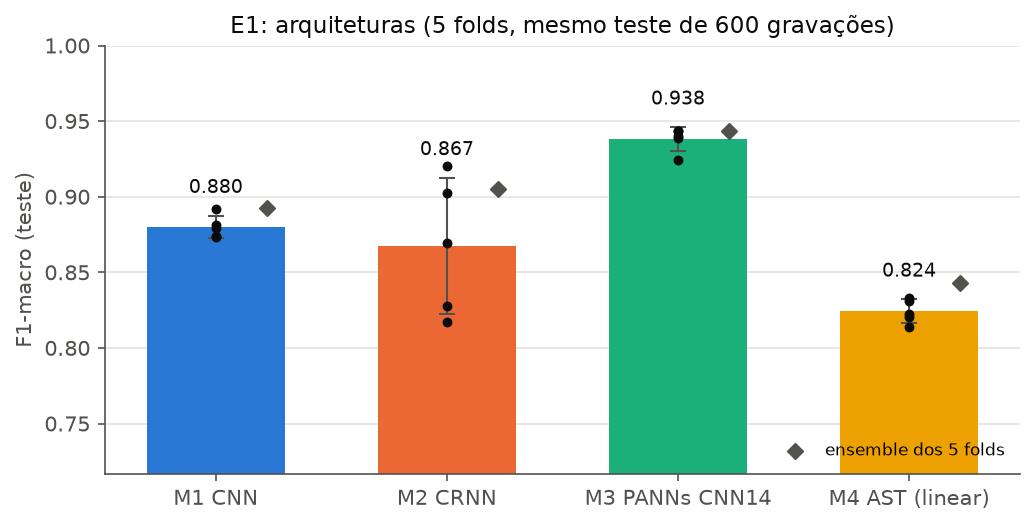
\includegraphics[width=\columnwidth]{e1_f1_teste.png}
\caption{E1: F1-macro no teste. Pontos: os 5 \textit{folds}; losango: \textit{ensemble}.}
\label{fig:e1}
\end{figure}

As comparações pareadas (Tabela~\ref{tab:comp}) confirmam: o M3 vence o M1 nos 5 \textit{folds}, com intervalo de 95\% longe de zero. O M4 perde do M1 nos 5. Entre M2 e M1 o resultado é inconclusivo. \textbf{H1 é apoiada para o ajuste fino e rejeitada para o pré-treino congelado}: no AudioSet as aves formam praticamente uma única classe, e o \textit{embedding} genérico não separa espécies sem adaptação. \textbf{H2 não é apoiada}: com janelas de 5~s e \textit{pooling} global no tempo, a CNN já captura o padrão do canto, curto e repetitivo.

\begin{table}[htbp]
\caption{Comparações pareadas no teste}
\label{tab:comp}
\centering
\footnotesize
\setlength{\tabcolsep}{4pt}
\begin{tabular}{@{}lccc@{}}
\toprule
\textbf{A $-$ B} & \textbf{dif. por fold} & \textbf{A vence} & \textbf{IC 95\% (ensembles)} \\
\midrule
M3 $-$ M1 & $+$0,058 & 5/5 & [$+$0,029; $+$0,076] \\
M3 $-$ M2 & $+$0,071 & 5/5 & [$+$0,017; $+$0,060] \\
M4 $-$ M1 & $-$0,056 & 0/5 & [$-$0,081; $-$0,020] \\
M2 $-$ M1 & $-$0,013 & 2/5 & [$-$0,005; $+$0,031] \\
\bottomrule
\end{tabular}
\end{table}

\subsection{E2 e E3: aumento de dados e ruído (H3)}

Na Parte~1, cada técnica isolada melhorou o M1 em 2{,}6 a 3{,}8 pontos (sem aumento: $0{,}844$; SpecAugment: $0{,}870$; \textit{mixup}: $0{,}872$; ruído: $0{,}882$; as três: $0{,}876$, média de 3 sementes). Na Parte~2, o aumento elevou o M2 de $0{,}779$ para $0{,}869$ (+9 pontos) e o M3 de $0{,}926$ para $0{,}939$: a CRNN é a que mais depende dele, e o pré-treino já fornece boa parte da robustez.

Sob ruído (Fig.~\ref{fig:e3}), a queda do teste limpo para 0~dB com aumento contra sem aumento foi de $-3{,}0$ contra $-5{,}9$ pontos no M1, $-2{,}4$ contra $-6{,}5$ no M2 e $-2{,}1$ contra $-6{,}3$ no M3. O M4, sem aumento possível, perde $9{,}6$ pontos. \textbf{H3 é apoiada}: o aumento reduz a queda a menos da metade. O M3 com aumento a 0~dB ($0{,}918$) supera o M1 em áudio limpo.

\begin{figure}[htbp]
\centering
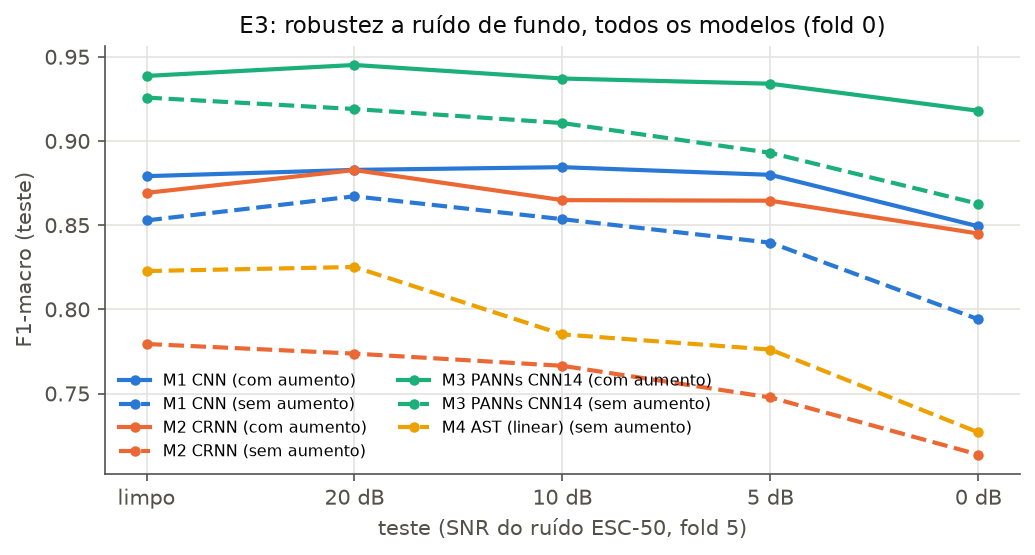
\includegraphics[width=\columnwidth]{e3b_snr.png}
\caption{E3: F1-macro no teste com ruído da ESC-50 (clipes nunca vistos no treino), com e sem aumento.}
\label{fig:e3}
\end{figure}

\subsection{E4: eficiência de dados (H1)}

Com 25\%, 50\% e 100\% das gravações, o M1 obtém $0{,}704$, $0{,}809$ e $0{,}879$; o M3, $0{,}814$, $0{,}882$ e $0{,}939$; o M4, $0{,}750$, $0{,}790$ e $0{,}823$ (Fig.~\ref{fig:e4}). A vantagem do M3 sobre o M1 cresce de 6 pontos (100\%) para 11 pontos (25\%), e \textbf{com metade dos dados o M3 já supera o M1 com todos}, o que apoia a segunda metade de H1. O M4, com representação fixa, é o que menos depende de dados.

\begin{figure}[htbp]
\centering
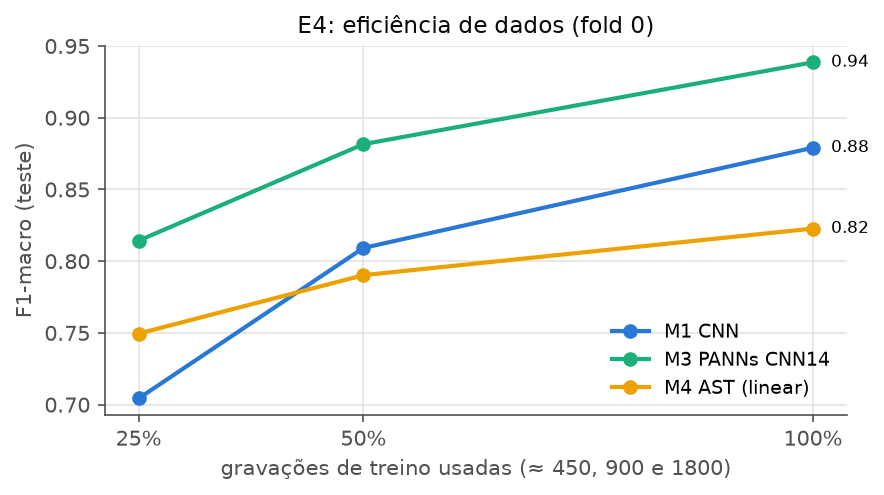
\includegraphics[width=\columnwidth]{e4_fracao.png}
\caption{E4: F1-macro no teste em função da fração de gravações de treino.}
\label{fig:e4}
\end{figure}

\subsection{Análises}

O M3 é melhor que o M1 em 16 das 20 espécies, com ganho maior nas mais difíceis (\textit{White-breasted Wood-Wren}: $0{,}73 \rightarrow 0{,}88$). O par mais confundido pelo M3 é \textit{Buff-throated Saltator} $\times$ \textit{White-breasted Wood-Wren}, duas espécies de canto assobiado na mesma faixa de frequência. O t-SNE~\cite{vandermaaten2008tsne} dos \textit{embeddings} mostra grupos mais compactos no M3 e, nos dois modelos, um núcleo misturado de janelas sem canto, consequência do rótulo fraco. O Grad-CAM~\cite{selvaraju2017gradcam} (Fig.~\ref{fig:gradcam}) indica que os modelos se concentram nas notas do canto, e não no ruído de fundo.

\begin{figure}[htbp]
\centering
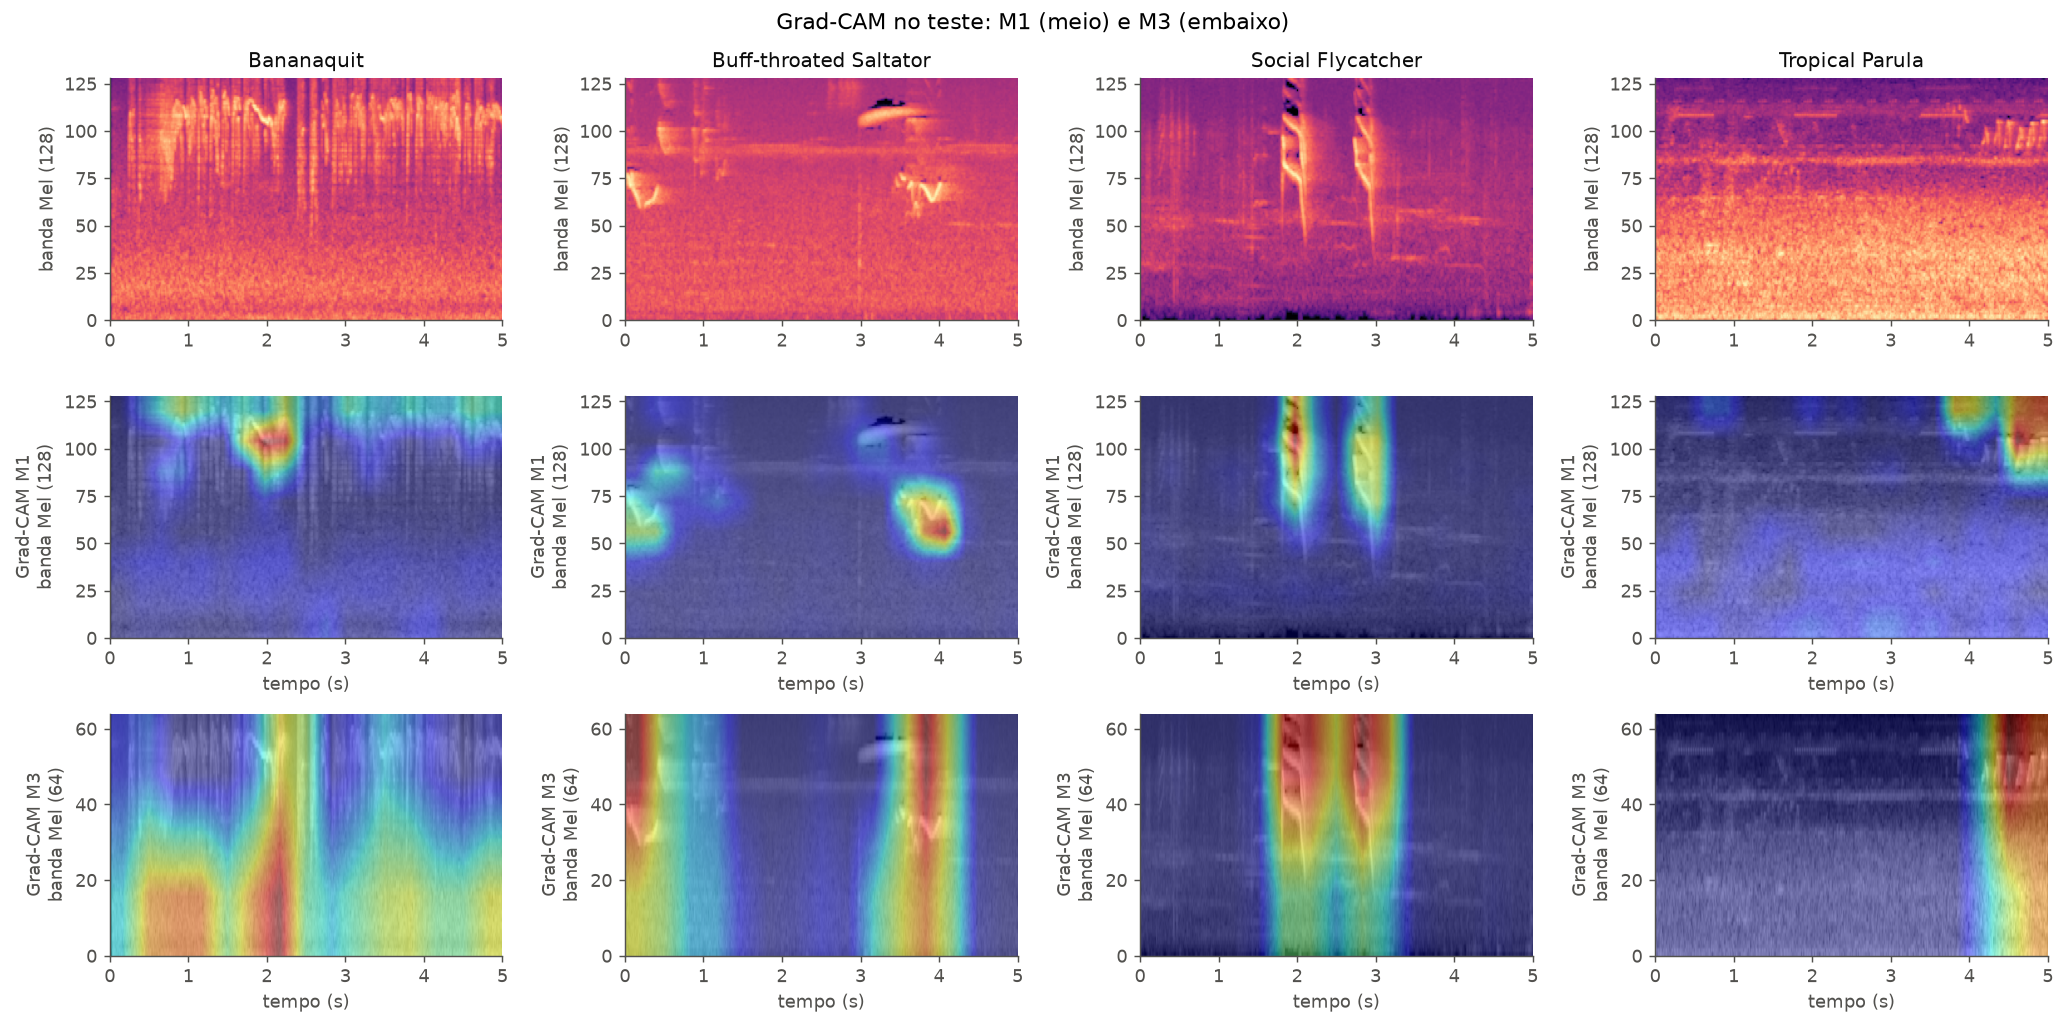
\includegraphics[width=\columnwidth]{gradcam_M1_M3.png}
\caption{Grad-CAM em quatro janelas de teste: log-Mel (em cima), M1 (meio) e M3 (embaixo).}
\label{fig:gradcam}
\end{figure}

% ---------------------------------------------------------------
\section{Melhorias (E5)}

\textbf{Linha de base clássica (M0).} Com 104 características por janela (MFCC~\cite{davis1980mfcc} e deltas, centroide, largura de banda, \textit{rolloff}, \textit{flatness} e energia por faixa) e três famílias de classificadores~\cite{pedregosa2011sklearn}, o melhor resultado foi F1 de $0{,}550$ no teste. As redes ganham 33 pontos (M1) e 39 pontos (M3): estatísticas resumidas da janela perdem a forma tempo-frequência das notas.

\textbf{Técnicas avaliadas.} A Tabela~\ref{tab:e5} resume as técnicas mantidas na validação e o seu resultado no teste. Não ajudaram: TTA por deslocamento no tempo, agregação das janelas por máximo ou \textit{top-3}, \textit{label smoothing}~\cite{szegedy2016inception}, treino mais longo, destilação do M3 no M1~\cite{hinton2015distilling} e ajuste do M3 em duas fases. Várias técnicas melhoraram a validação em cerca de 1 ponto e \textbf{não} melhoraram o teste: com 480 gravações de validação, 1 ponto equivale a cerca de 5 gravações. Só os ganhos grandes se confirmaram.

\begin{table}[htbp]
\caption{E5: técnicas mantidas e efeito no teste}
\label{tab:e5}
\centering
\footnotesize
\setlength{\tabcolsep}{3pt}
\begin{tabular}{@{}>{\raggedright\arraybackslash}p{3.7cm}cc@{}}
\toprule
\textbf{Técnica (base)} & \textbf{Base} & \textbf{Técnica} \\
\midrule
PCEN no lugar do log (M1) & 0,879 & \textbf{0,902} \\
\quad mesma, teste a 0~dB & 0,849 & \textbf{0,875} \\
EfficientNet-B0 ImageNet (M1) & 0,879 & 0,923 \\
AST com 2 blocos ajustados (M4) & 0,823 & 0,853 \\
\textit{Ensemble} ponderado M1+M2+M3 (M3) & 0,939 & 0,944 \\
Divisão por autor (M1, medição) & 0,879 & 0,842 \\
\bottomrule
\end{tabular}
\end{table}

A PCEN~\cite{wang2017pcen} normaliza cada banda pela própria energia recente, realça eventos curtos e atenua o ruído estacionário, o que explica o ganho também a 0~dB. A EfficientNet-B0~\cite{tan2019efficientnet} pré-treinada no ImageNet~\cite{deng2009imagenet} mostra que qualquer pré-treino ajuda bastante (+4{,}4 pontos), mas o pré-treino em áudio do M3 acrescenta outros 1{,}6 pontos.

\textbf{Calibração.} O \textit{ensemble} se mostrou pouco confiante: confiança média de 0{,}71 para acurácia de 0{,}94. Um \textit{temperature scaling}~\cite{guo2017calibration} com $T = 0{,}53$, ajustado na validação, reduziu o ECE do teste de $0{,}230$ para $0{,}027$, sem alterar o F1.

% ---------------------------------------------------------------
\section{M6: uma CNN guiada pelos resultados}
\label{sec:m6}

O M6 junta, numa CNN do porte do M1, peças conhecidas escolhidas a partir dos nossos resultados:

\begin{enumerate}
  \item \textbf{PCEN treinável} por banda, como no LEAF~\cite{zeghidour2021leaf}, inicializada na PCEN fixa, que foi a melhor técnica do E5;
  \item \textbf{blocos residuais}~\cite{he2016resnet} com \textit{Squeeze-and-Excitation}~\cite{hu2018se}, com larguras 16-32-64-128 para manter o porte do M1;
  \item um \textbf{canal com a posição da banda}, como no CoordConv~\cite{liu2018coordconv}, pois cada espécie canta numa faixa própria;
  \item \textbf{atenção com portas sobre as janelas} da gravação~\cite{ilse2018attention}, por causa do rótulo fraco, treinada numa segunda etapa com o corpo congelado.
\end{enumerate}

A ablação adiciona uma peça por vez e só a mantém se melhorar a validação (Fig.~\ref{fig:m6}). A PCEN treinável sobe a validação de $0{,}869$ para $0{,}879$. Os blocos residuais dão o grande salto, para $0{,}931$, e a $0{,}924$ no teste. O canal de frequência piora ($0{,}914$) e é descartado. A atenção sobre a melhor base empata na validação ($0{,}932$), mas fica 1 ponto abaixo no teste ($0{,}914$). Pelo protocolo, o M6 final (com atenção) é o escolhido na validação e chega a $0{,}914$ no teste limpo e a $0{,}920$ a 0~dB, no nível do M3 ($0{,}918$).

\begin{figure}[htbp]
\centering
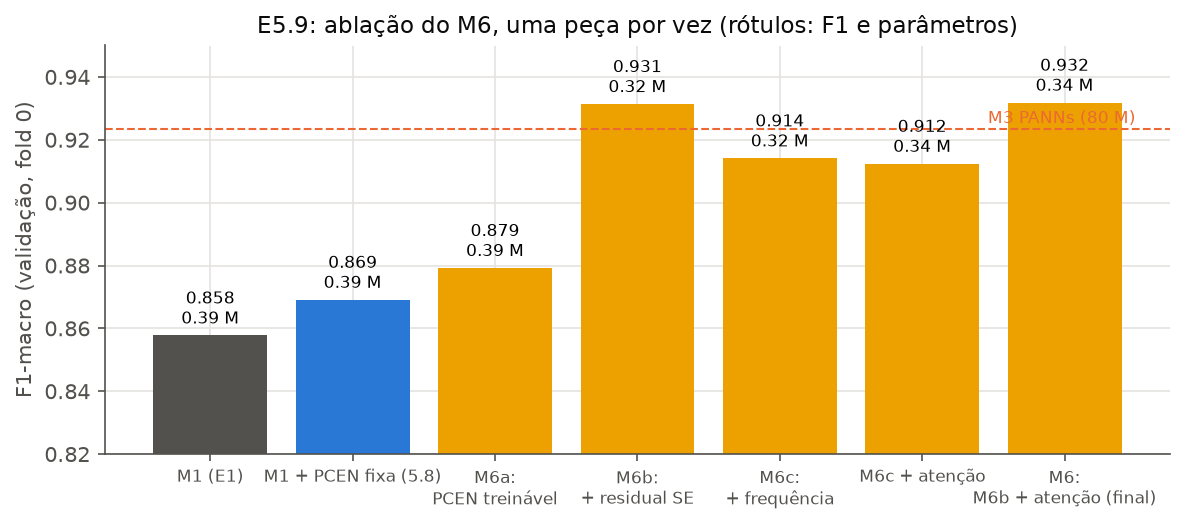
\includegraphics[width=\columnwidth]{e5_m6_ablacao.png}
\caption{Ablação do M6 (validação do \textit{fold} 0). A linha tracejada é o M3, com 80 milhões de parâmetros.}
\label{fig:m6}
\end{figure}

O M6b, sem pré-treino e com 0{,}32 milhão de parâmetros, empata com a EfficientNet do ImageNet (0{,}923; 12 vezes mais parâmetros) e fica a 1{,}5 ponto do M3 (250 vezes mais). A PCEN aprendeu sozinha a remover o fundo mais depressa abaixo de 1~kHz (constante de tempo de 0{,}26 a 0{,}37~s e compressão mais forte) e a preservar a faixa dos cantos, de 2 a 10~kHz (Fig.~\ref{fig:pcen}). A atenção concentrou o peso em poucas janelas, descartando evidência útil, o que ajuda a explicar por que não superou a média simples.

\begin{figure*}[t]
\centering
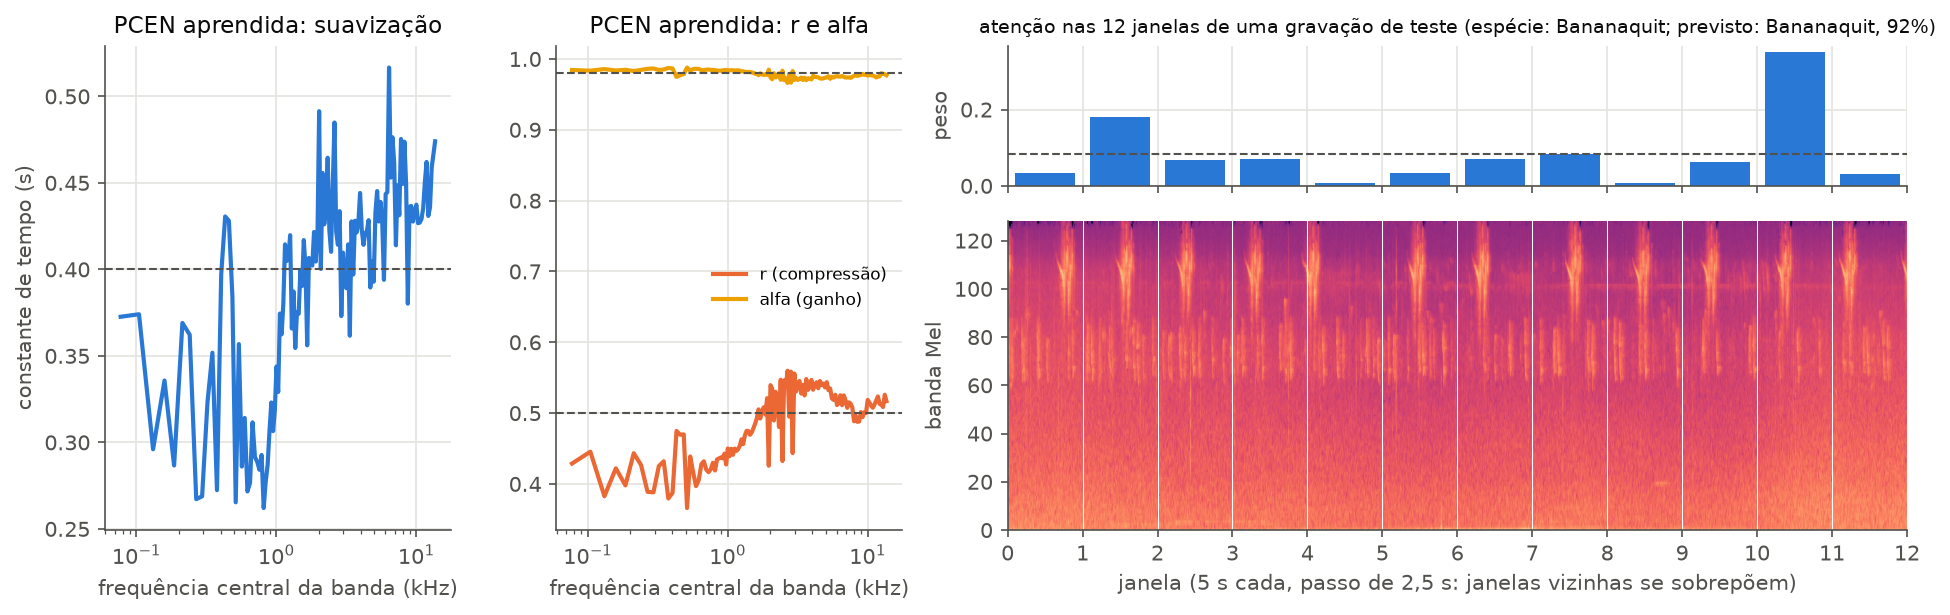
\includegraphics[width=0.92\textwidth]{e5_m6_pcen_atencao.png}
\caption{O que o M6 aprendeu. Esquerda: parâmetros da PCEN por banda (tracejado: PCEN fixa inicial). Direita: pesos da atenção nas 12 janelas de uma gravação de teste.}
\label{fig:pcen}
\end{figure*}

% ---------------------------------------------------------------
\section{Sistema final}

O sistema final combina o M1 com PCEN (peso $0{,}35$), o M2 ($0{,}10$) e o M3 ($0{,}55$), com pesos escolhidos na validação e temperatura de calibração $T = 0{,}46$. Ele atinge \textbf{F1-macro de 0{,}950} no teste, com \textit{top-1} de $0{,}950$ e \textit{top-3} de $0{,}985$. Os pesos finais e um comando de inferência (\texttt{python -m birdclef.inferencia arquivo.ogg}) estão no repositório.

% ---------------------------------------------------------------
\section{Limitações}
\label{sec:limitacoes}

\begin{itemize}
  \item \textbf{Dados curados:} 20 espécies comuns, gravações boas e classes equilibradas. Gravações de campo, com várias aves sobrepostas e espécies raras, são bem mais difíceis.
  \item \textbf{Gravadores repetidos:} 90\% das gravações de teste têm o autor no treino. Refazendo a divisão por autor, o M1 cai 3{,}7 pontos. O efeito é menor que as diferenças entre modelos, mas os números absolutos são otimistas.
  \item \textbf{Ruído sintético:} a mistura com a ESC-50 a SNR controlada não equivale a ruído real de campo.
  \item \textbf{Variância:} E2b, E3b, E4 e as variantes do E5 usam um treino por configuração. Diferenças de cerca de 1 ponto não são conclusivas.
  \item \textbf{Hardware:} com uma GPU de 4~GB, o AST não pôde ser ajustado por completo, o que torna desigual a comparação com o M4.
\end{itemize}

Os resultados servem para comparar modelos sob as mesmas condições, e não para estimar o desempenho em campo.

% ---------------------------------------------------------------
\section{Conclusão}

O pré-treino em áudio com ajuste fino foi o fator de maior impacto (H1), sobretudo com poucos dados. Usado congelado, porém, o modelo pré-treinado ficou abaixo de uma CNN pequena. Modelar o tempo com uma GRU não trouxe ganho em janelas de 5~s (H2). O aumento de dados foi barato e eficaz em todos os modelos, reduzindo à metade a queda sob ruído (H3). Na etapa de melhorias, o processamento de sinais clássico mostrou valor dentro da rede: a PCEN foi a melhor técnica, e a CNN própria M6, construída a partir dos resultados, alcançou o desempenho de um modelo pré-treinado 12 vezes maior. Como trabalhos futuros, propomos avaliar em gravações de campo multirrótulo, ampliar o número de espécies, adotar a divisão por gravador como padrão e combinar a PCEN com modelos pré-treinados específicos de aves.

% ---------------------------------------------------------------
\section*{Apresentação}

{\raggedright A apresentação do projeto foi feita em vídeo. Os slides usados estão no repositório, no arquivo \url{apresentacao/slides.pdf}.\par}

% ---------------------------------------------------------------
\begin{thebibliography}{00}

\bibitem{stowell2022} D. Stowell, ``Computational bioacoustics with deep learning: a review and roadmap,'' \textit{PeerJ}, vol. 10, e13152, 2022.

\bibitem{kahl2021birdnet} S. Kahl, C. M. Wood, M. Eibl, and H. Klinck, ``BirdNET: A deep learning solution for avian diversity monitoring,'' \textit{Ecological Informatics}, vol. 61, 101236, 2021.

\bibitem{hershey2017} S. Hershey \textit{et al.}, ``CNN architectures for large-scale audio classification,'' in \textit{Proc. IEEE ICASSP}, 2017, pp. 131--135.

\bibitem{choi2017crnn} K. Choi, G. Fazekas, M. Sandler, and K. Cho, ``Convolutional recurrent neural networks for music classification,'' in \textit{Proc. IEEE ICASSP}, 2017, pp. 2392--2396.

\bibitem{gemmeke2017audioset} J. F. Gemmeke \textit{et al.}, ``Audio Set: An ontology and human-labeled dataset for audio events,'' in \textit{Proc. IEEE ICASSP}, 2017, pp. 776--780.

\bibitem{kong2020panns} Q. Kong, Y. Cao, T. Iqbal, Y. Wang, W. Wang, and M. D. Plumbley, ``PANNs: Large-scale pretrained audio neural networks for audio pattern recognition,'' \textit{IEEE/ACM Trans. Audio, Speech, Lang. Process.}, vol. 28, pp. 2880--2894, 2020.

\bibitem{gong2021ast} Y. Gong, Y.-A. Chung, and J. Glass, ``AST: Audio Spectrogram Transformer,'' in \textit{Proc. Interspeech}, 2021, pp. 571--575.

\bibitem{kahl2021birdclef} S. Kahl \textit{et al.}, ``Overview of BirdCLEF 2021: Bird call identification in soundscape recordings,'' in \textit{Working Notes of CLEF 2021}, CEUR Workshop Proceedings, 2021.

\bibitem{park2019specaugment} D. S. Park \textit{et al.}, ``SpecAugment: A simple data augmentation method for automatic speech recognition,'' in \textit{Proc. Interspeech}, 2019, pp. 2613--2617.

\bibitem{zhang2018mixup} H. Zhang, M. Cisse, Y. N. Dauphin, and D. Lopez-Paz, ``mixup: Beyond empirical risk minimization,'' in \textit{Proc. ICLR}, 2018.

\bibitem{wang2017pcen} Y. Wang, P. Getreuer, T. Hughes, R. F. Lyon, and R. A. Saurous, ``Trainable frontend for robust and far-field keyword spotting,'' in \textit{Proc. IEEE ICASSP}, 2017, pp. 5670--5674.

\bibitem{zeghidour2021leaf} N. Zeghidour, O. Teboul, F. de Chaumont Quitry, and M. Tagliasacchi, ``LEAF: A learnable frontend for audio classification,'' in \textit{Proc. ICLR}, 2021.

\bibitem{birdclef2025} BirdCLEF+ 2025, Kaggle, 2025. [Online]. Disponível em: \url{https://www.kaggle.com/competitions/birdclef-2025}

\bibitem{xenocanto} Xeno-canto Foundation, ``xeno-canto: Sharing wildlife sounds from around the world.'' [Online]. Disponível em: \url{https://xeno-canto.org}

\bibitem{piczak2015esc} K. J. Piczak, ``ESC: Dataset for environmental sound classification,'' in \textit{Proc. 23rd ACM Int. Conf. Multimedia}, 2015, pp. 1015--1018.

\bibitem{loshchilov2019adamw} I. Loshchilov and F. Hutter, ``Decoupled weight decay regularization,'' in \textit{Proc. ICLR}, 2019.

\bibitem{vandermaaten2008tsne} L. van der Maaten and G. Hinton, ``Visualizing data using t-SNE,'' \textit{J. Mach. Learn. Res.}, vol. 9, pp. 2579--2605, 2008.

\bibitem{selvaraju2017gradcam} R. R. Selvaraju \textit{et al.}, ``Grad-CAM: Visual explanations from deep networks via gradient-based localization,'' in \textit{Proc. IEEE ICCV}, 2017, pp. 618--626.

\bibitem{davis1980mfcc} S. Davis and P. Mermelstein, ``Comparison of parametric representations for monosyllabic word recognition in continuously spoken sentences,'' \textit{IEEE Trans. Acoust., Speech, Signal Process.}, vol. 28, no. 4, pp. 357--366, 1980.

\bibitem{pedregosa2011sklearn} F. Pedregosa \textit{et al.}, ``Scikit-learn: Machine learning in Python,'' \textit{J. Mach. Learn. Res.}, vol. 12, pp. 2825--2830, 2011.

\bibitem{szegedy2016inception} C. Szegedy, V. Vanhoucke, S. Ioffe, J. Shlens, and Z. Wojna, ``Rethinking the Inception architecture for computer vision,'' in \textit{Proc. IEEE CVPR}, 2016, pp. 2818--2826.

\bibitem{hinton2015distilling} G. Hinton, O. Vinyals, and J. Dean, ``Distilling the knowledge in a neural network,'' arXiv:1503.02531, 2015.

\bibitem{tan2019efficientnet} M. Tan and Q. V. Le, ``EfficientNet: Rethinking model scaling for convolutional neural networks,'' in \textit{Proc. ICML}, 2019, pp. 6105--6114.

\bibitem{deng2009imagenet} J. Deng, W. Dong, R. Socher, L.-J. Li, K. Li, and L. Fei-Fei, ``ImageNet: A large-scale hierarchical image database,'' in \textit{Proc. IEEE CVPR}, 2009, pp. 248--255.

\bibitem{guo2017calibration} C. Guo, G. Pleiss, Y. Sun, and K. Q. Weinberger, ``On calibration of modern neural networks,'' in \textit{Proc. ICML}, 2017, pp. 1321--1330.

\bibitem{he2016resnet} K. He, X. Zhang, S. Ren, and J. Sun, ``Deep residual learning for image recognition,'' in \textit{Proc. IEEE CVPR}, 2016, pp. 770--778.

\bibitem{hu2018se} J. Hu, L. Shen, and G. Sun, ``Squeeze-and-excitation networks,'' in \textit{Proc. IEEE CVPR}, 2018, pp. 7132--7141.

\bibitem{liu2018coordconv} R. Liu \textit{et al.}, ``An intriguing failing of convolutional neural networks and the CoordConv solution,'' in \textit{Proc. NeurIPS}, 2018.

\bibitem{ilse2018attention} M. Ilse, J. M. Tomczak, and M. Welling, ``Attention-based deep multiple instance learning,'' in \textit{Proc. ICML}, 2018, pp. 2127--2136.

\end{thebibliography}

\end{document}
